\documentclass[tikz,border=6pt]{standalone}
% =============================================================================
%  PREAMBULE COMMUN DES SCHEMAS DU SUPPORT DE SOUTENANCE (ENSAE, octobre 2026)
%
%  Les schemas sont des VISUELS DE DIAPOSITIVE, pas des figures de donnees : ils
%  prennent donc la palette du gabarit de presentation Nexialog, recopiee de
%  build_soutenance_ppt.py, et jamais celle de style_nexialog.py, qui reste la
%  source unique des couleurs des figures du memoire.
%
%  AUCUN NOMBRE DE RESULTAT N'Y FIGURE. Un nombre dessine dans une image echappe
%  au controle du support, qui verifie chaque nombre de texte contre le rapport.
%  Les schemas portent des symboles et des equations, recopiees du rapport.
%
%  Polices : Segoe UI pour le texte, comme le corps du gabarit ; Latin Modern Math
%  pour les formules, celle du rapport. Chaque schema se dessine A SA TAILLE FINALE
%  sur la diapositive, si bien qu'un corps de 14 pt ici vaut 14 pt a l'ecran.
% =============================================================================
\usepackage{fontspec}
\usepackage{unicode-math}
\setmainfont{Segoe UI}
\setsansfont{Segoe UI}
\setmathfont{latinmodern-math.otf}
\usetikzlibrary{positioning,arrows.meta,calc,fit,backgrounds,shapes.geometric,decorations.pathreplacing}

\definecolor{ardoise}{HTML}{223E55}   % titres et aplats du gabarit
\definecolor{profond}{HTML}{192E3F}
\definecolor{acier}{HTML}{435B6E}
\definecolor{encre}{HTML}{122738}     % texte courant
\definecolor{gris}{HTML}{595959}      % texte secondaire
\definecolor{accent}{HTML}{B10031}    % rouge de marque
\definecolor{clair}{HTML}{F2F2F2}
\definecolor{filet}{HTML}{D9D9D9}

\newcommand{\corps}{\fontsize{14}{17}\selectfont}
\newcommand{\petit}{\fontsize{12}{14.5}\selectfont}
\newcommand{\grand}{\fontsize{16}{19}\selectfont}
\tikzset{
  >={Stealth[length=7pt,width=6pt]},
  bloc/.style={draw=ardoise, line width=0.9pt, fill=white, rounded corners=3pt,
               inner sep=6pt, align=center, text=encre, font=\corps},
  bloc plein/.style={fill=ardoise, draw=ardoise, rounded corners=3pt, inner sep=6pt,
               align=center, text=white, font=\corps\bfseries},
  bloc accent/.style={fill=accent, draw=accent, rounded corners=3pt, inner sep=6pt,
               align=center, text=white, font=\corps\bfseries},
  fleche/.style={->, line width=1.3pt, draw=acier},
  fleche accent/.style={->, line width=1.6pt, draw=accent},
  legende/.style={font=\petit, text=gris, align=center},
}

% -----------------------------------------------------------------------------
%  Schema « une matrice et sa transposee » (support de soutenance ENSAE).
%  Taille finale : 11,4 x 3,9 pouces. Aucun nombre de resultat.
%  Sources des libelles et de la formule :
%   - decomposition : chapitres_sfe/08_identification_partielle.tex, l. 26-28 ;
%   - « une matrice et sa transposee », « capital et decision differents » :
%     chapitres_sfe/00_introduction.tex l. 63-65 et 01_contexte.tex l. 312-314 ;
%   - « meme co-occurrence au premier ordre » : proposition prop:nonid,
%     chapitres_sfe/05_cascade.tex l. 288-303, enonce (i) l. 298-299 ;
%   - « co-occurrence, identifiee » / « direction, non identifiee » :
%     chapitres_sfe/08_identification_partielle.tex l. 29 ;
%   - « donnees publiques agregees » : chapitres_sfe/07_identifiabilite.tex l. 21-22.
%  Le schema ne dit pas que la direction est inobservable : la loi jointe des
%  piliers touches distingue une matrice de sa transposee (prop:nonid (ii) ;
%  05_cascade.tex l. 331 ; 10_robustesse.tex l. 318-319 ; conclusion.tex
%  l. 60-61). Il montre ce que voient les donnees publiques agregees.
% -----------------------------------------------------------------------------
\begin{document}
\begin{tikzpicture}[
  pilier/.style={circle, fill=ardoise, draw=ardoise, text=white, font=\corps\bfseries,
                 minimum size=1.05cm, inner sep=0pt},
  fort/.style={-{Stealth[length=10pt,width=9pt]}, line width=3.2pt, draw=ardoise,
               shorten <=0.6cm, shorten >=0.6cm},
  faible/.style={-{Stealth[length=7pt,width=6pt]}, line width=1.2pt, draw=ardoise,
               shorten <=0.6cm, shorten >=0.6cm},
  arete/.style={line width=2.2pt, draw=ardoise, shorten <=1pt, shorten >=1pt},
  titre/.style={font=\corps\bfseries, text=ardoise, anchor=base},
  formule/.style={font=\grand, text=encre, anchor=base},
  sens/.style={font=\corps, text=gris, anchor=base},
]
\def\ecart{0.15cm}
% \paire{u}{v}{style de u vers v}{style de v vers u} : deux fleches paralleles,
% chacune sur sa gauche, si bien qu'une paire garde ses deux voies d'un panneau a l'autre
\newcommand{\paire}[4]{%
  \draw[#3] ($(#1.center)!\ecart!90:(#2.center)$) -- ($(#2.center)!\ecart!-90:(#1.center)$);
  \draw[#4] ($(#2.center)!\ecart!90:(#1.center)$) -- ($(#1.center)!\ecart!-90:(#2.center)$);
}
% \trio{prefixe}{x du centre} : P1 en haut, P2 en bas a gauche, P4 en bas a droite
\newcommand{\trio}[2]{%
  \node[pilier] (#1p1) at (#2, 6.95) {P1};
  \node[pilier] (#1p2) at ($(#2,3.45)+(-2.25,0)$) {P2};
  \node[pilier] (#1p4) at ($(#2,3.45)+(2.25,0)$) {P4};
}

% cadre exact de la figure (11,4 x 3,9 pouces, bordure de 6 pt comprise)
\useasboundingbox (0,0) rectangle (28.53,9.48);

% ---- d'abord la decomposition (consigne d'Hugo : S/A d'abord, puis les schemas)
\node[formule] (fW) at (6.61, 8.45) {$W \;=\; S + A$};
\node[formule] (fS) at (13.56, 8.45) {$S = \tfrac{1}{2}(W + W^{\top})$};
\node[formule] (fA) at (20.96, 8.45) {$A = \tfrac{1}{2}(W - W^{\top})$};
\node[sens] at (6.61, 7.45) {toute matrice réelle};
\node[sens] at (13.56, 7.45) {co-occurrence, identifiable};
\node[sens] at (20.96, 7.45) {direction, non identifiée};

% ---- puis les schemas, decales sous la decomposition -------------------------
\begin{scope}[yshift=-2.35cm]
% ---- les deux matrices, regroupees ------------------------------------------
\fill[clair, rounded corners=4pt] (0,2.45) rectangle (16.6,8.95);

\trio{a}{3.2}
\node[titre] at (3.2, 8.15) {Une matrice $W$};
\paire{ap1}{ap2}{fort}{faible}
\paire{ap1}{ap4}{fort}{faible}
\paire{ap4}{ap2}{fort}{faible}

\trio{b}{13.4}
\node[titre] at (13.4, 8.15) {Sa transposée $W^{\top}$};
\paire{bp1}{bp2}{faible}{fort}
\paire{bp1}{bp4}{faible}{fort}
\paire{bp4}{bp2}{faible}{fort}

% ---- le message : une matrice et sa transposee donnent un capital different -
% le signe est trace au trait, au poids du libelle en gras (le glyphe de
% Latin Modern Math, trop fin a cette taille, se perdait a cote du texte)
\begin{scope}[draw=accent, line width=2.4pt, line cap=round]
  \draw (7.72, 5.92) -- (8.88, 5.92);
  \draw (7.72, 6.30) -- (8.88, 6.30);
  \draw (8.02, 5.50) -- (8.58, 6.72);
\end{scope}
\node[text=accent, font=\corps\bfseries, align=center, anchor=north] at (8.3, 5.28)
  {capital\\et décision\\différents};

% ---- ce que voient les donnees -----------------------------------------------
\trio{c}{25.25}
\node[titre] at (25.25, 8.8) {Ce que voient les données};
\node[titre] at (25.25, 8.15) {publiques agrégées~: $S$};
\draw[arete] (cp1) -- (cp2);
\draw[arete] (cp1) -- (cp4);
\draw[arete] (cp4) -- (cp2);

\draw[fleche, line width=1.6pt] (16.85, 5.2) -- (23.25, 5.2)
  node[midway, above=3pt, font=\corps, text=encre] {même co-occurrence}
  node[midway, below=3pt, font=\corps, text=encre] {au premier ordre};
\end{scope}
\end{tikzpicture}
\end{document}
